\documentclass[10pt, a4paper]{article}
\usepackage[utf8x]{inputenc}            % Acentos, ñ, etc.
\usepackage{graphicx}                   % Gráficos
\usepackage[spanish]{babel}             % Macros en español
\usepackage{caratula}                   % Carátula
\usepackage{geometry}                   % Márgenes
\usepackage{listings}					% Codigo
\usepackage{float}						% Posicion de Imagenes
\begin{document}


%Caratula
\titulo{Trabajo Práctico 2}
\subtitulo{Cuatro en Línea}
\fecha{\today}
\materia{Aprendizaje Automático}
\integrante{Fernández, Gonzalo}{836/10}{gpfernandezflorio@gmail.com}
\integrante{Aleman, Damian}{377/10}{damianealeman@gmail.com}
\integrante{Pizzagalli, Matías}{257/10}{matipizza@gmail.com}


%Titulo e indice
\maketitle
\tableofcontents
\newpage


\section{Introducción}


En el presente trabajo práctico se analiza la estrategia de Aprendizaje Automático basado en Refuerzos para la implementación de un programa que simule un jugador del juego \texttt{Cuatro en Línea}. El algoritmo de aprendizaje utilizado es Q-Learning. Se utiliza como base una implementación en python del juego \texttt{Ta-Te-Ti} y un jugador Q-Learning para ese juego. A partir de esta implementación, se busca obtener un jugador para el \texttt{Cuatro en línea} que aprenda al mismo ritmo que el jugador de \texttt{Ta-Te-Ti}.


\subsection{Descripción del algoritmo de Q-Learning}


El primer paso para desarrollar un algoritmo Q-Learning es definir el espacio de estados y posibles acciones asociadas a tales estados. La implementación base de \texttt{Ta-Te-Ti} modela cada estado como una matriz de 3 por 3, representado el tablero en cada momento de la partida. Las acciones a tomar son cada ubicación libre del tablero, es decir, de la matriz.


En nuestro caso, cada configuración posible del tablero es un estado, es decir guardamos para cada posición del tablero si hay una ficha y de qué jugador. Muchos de esos estados son inalcanzables, ya que toda ficha debe estar inmediatamente por encima de otra ficha. Tampoco consideramos estados en los que hay cuatro fichas alineadas (ya sea de forma vertical, horizontal o diagonal), ya que en caso de suceder esto ya hay un ganador y el juego no continua.
Cada acción se corresponde con insertar una ficha en alguna de las columnas. La ficha será asignada a la fila inmediatamente superior a la fila donde estaba la ficha más arriba en la misma columna. En lugar de almacenar los estados como matrices, mantenemos un arreglo de Columnas, donde cada Columna no es más que una lista de caracteres, inicialmente vacía. Insertar una ficha en la columna $x$, consiste en agregar un caracter a la $x$-ésima lista del arreglo.

Al elegir esta forma de representacion del tablero conseguimos que no sea posible realizar movimientos invalidos, ya que siempre vamos a estar colocando fichas sobre otras fichas o sobre el fondo de la columna. Ademas, al no representar los lugares vacios el tablero ocupa a priori ocupa menos lugar en memoria, tomando como comparación la representacion matricial.


Las recompensas a las acciones tomadas se otorgan después de que juegue el rival, excepto en los casos en los que la partida finaliza.


En este trabajo observamos cuánto aprenden los modelos a partir de la cantidad de victorias que tienen contra otros modelos.
Hay muchos parámetros en el modelo que se pueden modificar:
$\epsilon$,  $\gamma$, $\alpha$, recompensa por ganar(perder o empatar) el partido, recompensa por un nuevo turno y la cantidad de iteraciones que se entrena.


\section{Experimentación}


\subsection{Experimentación Inicial}


Primero hicimos competir un Q-Learning Player (apartir de ahora QLP) contra un jugador Random y luego contra otro QLP. Para esta experimentación utilizamos los mismo parámetros que se usan en el ejemplo del \texttt{Ta-Te-Ti}, los cuales apartir de ahora llamamos parámetros por defecto. Estos parámetros por defecto son: $\alpha=0.3$,$\gamma=0.9$, $\epsilon=0.2$.

A continuación se muestran los resultados obtenidos.


\begin{figure}[H]
  \begin{minipage}[c]{1\textwidth}
	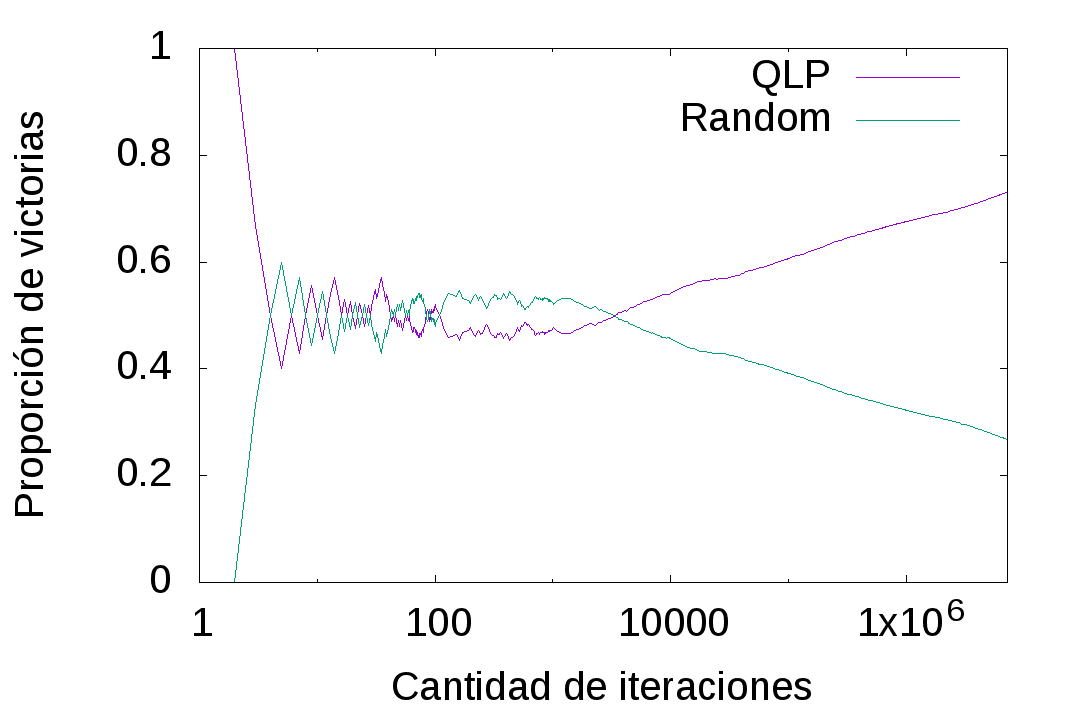
\includegraphics[scale=0.25]{Initial/QvR.png}
	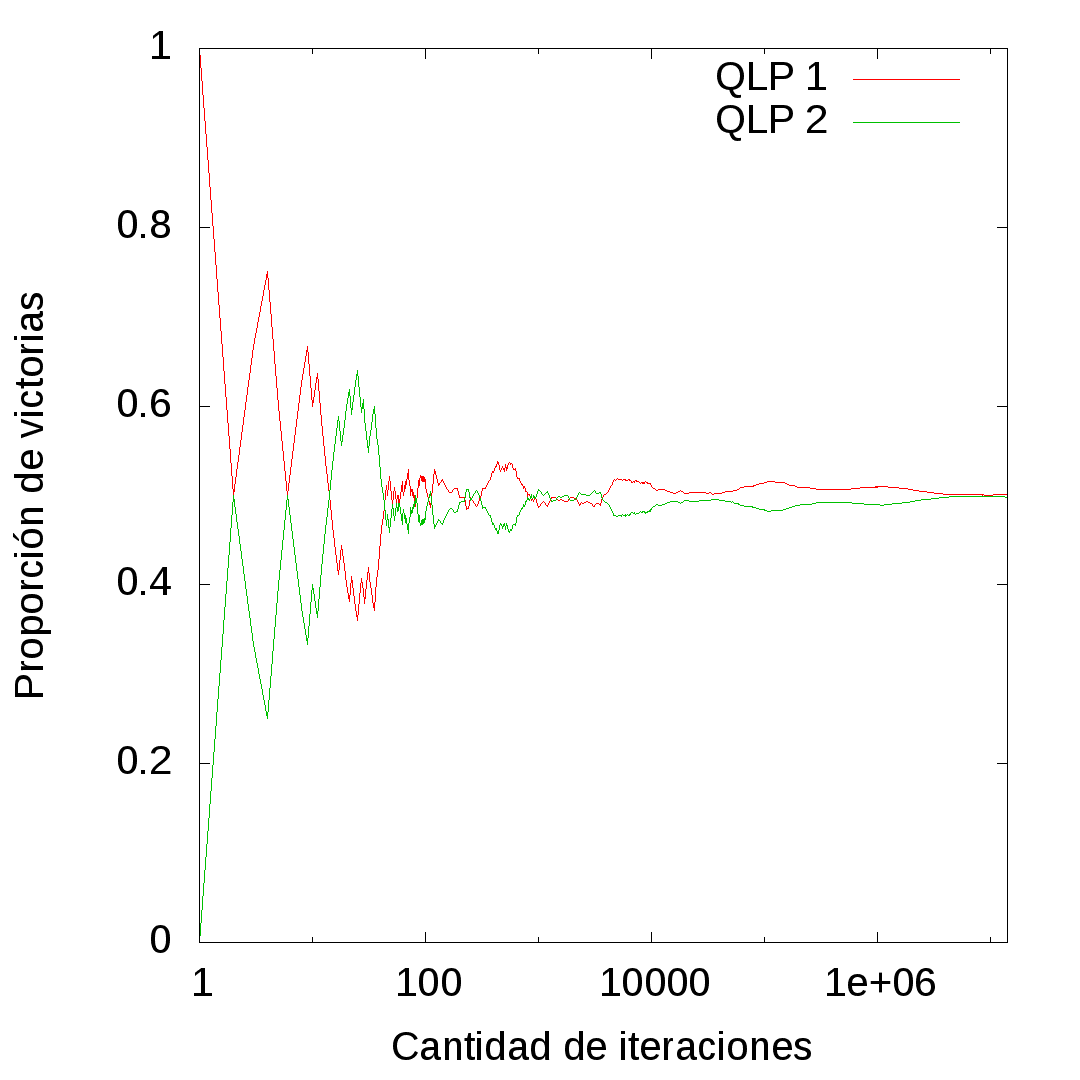
\includegraphics[scale=0.25]{Initial/QvQ.png}
  \end{minipage}
\end{figure}

En los gráficos podemos observar la proporción de victorias de cada jugador a medida que se van entrenando. De esta forma podemos ver como, al jugar contra un jugador Random, el jugador QLP aprende una estrategia para vencerlo y a partir de cierto punto, pareciera ganar la mayor parte de las veces, con lo cuál, su proporción de victorias sólo aumenta. En el caso de los dos jugadores QLP, parecieran retroalimentarse de forma que ambos tienden a ganar el $50\%$ de las veces. A diferencia de lo que se observó en el caso del \texttt{Ta-Te-Ti}, el ratio de empates es muy bajo.


\subsection{Ajuste de parámetros}


Experimentamos variando los parámetros $\alpha$, $\gamma$ y $\epsilon$ por separado, haciéndolo competir contra un jugador Random y contra un jugador QLP con los parámetros por defecto.
Cabe aclarar que mientras variamos un parámetro del modelo, los otros dos se fijan también en los valores por defecto ya mencionados.

\subsubsection{Experimentacion con Gamma}

\begin{figure}[H]
 \centering
  \begin{minipage}[c]{1\textwidth}
	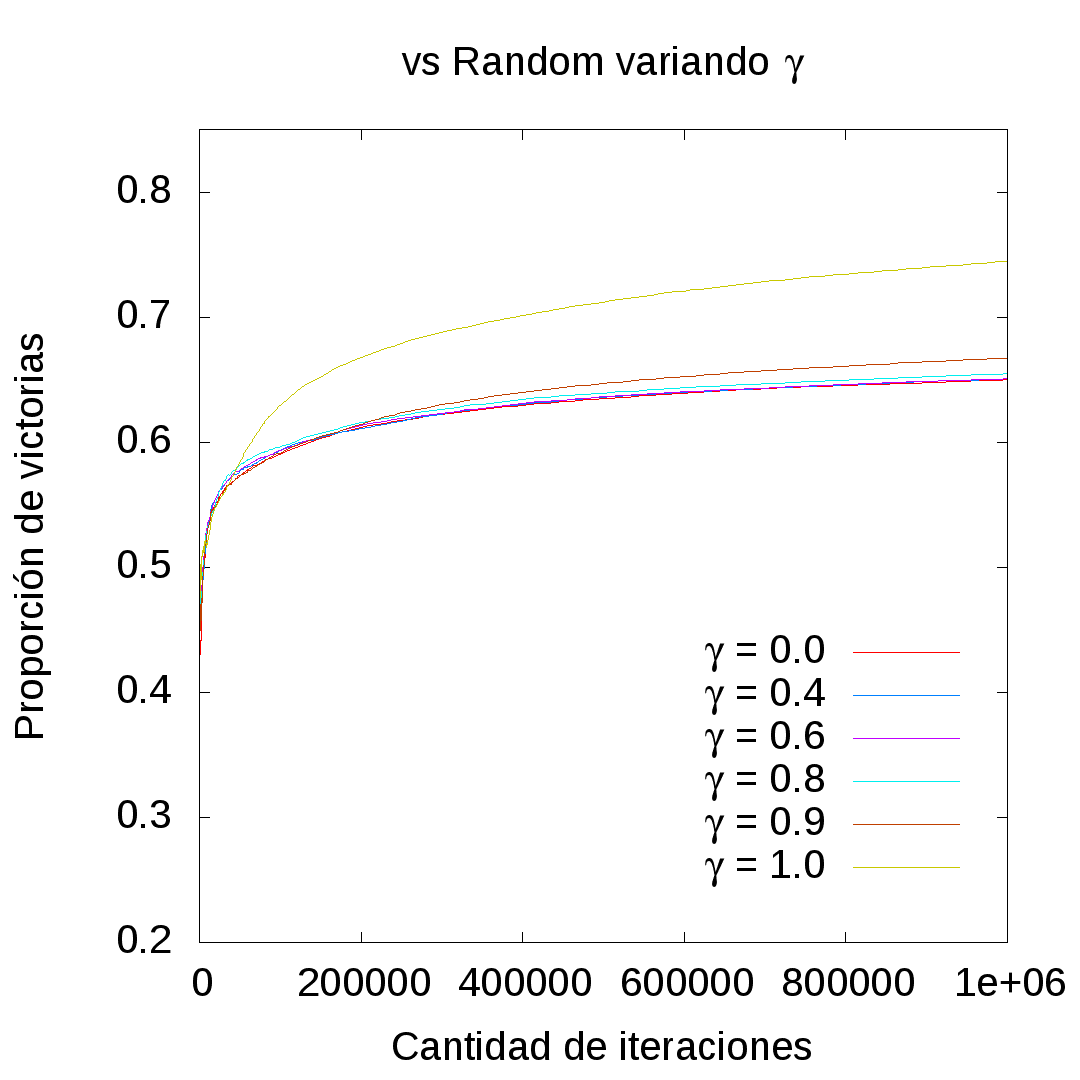
\includegraphics[scale=0.2]{GammaR.png}
	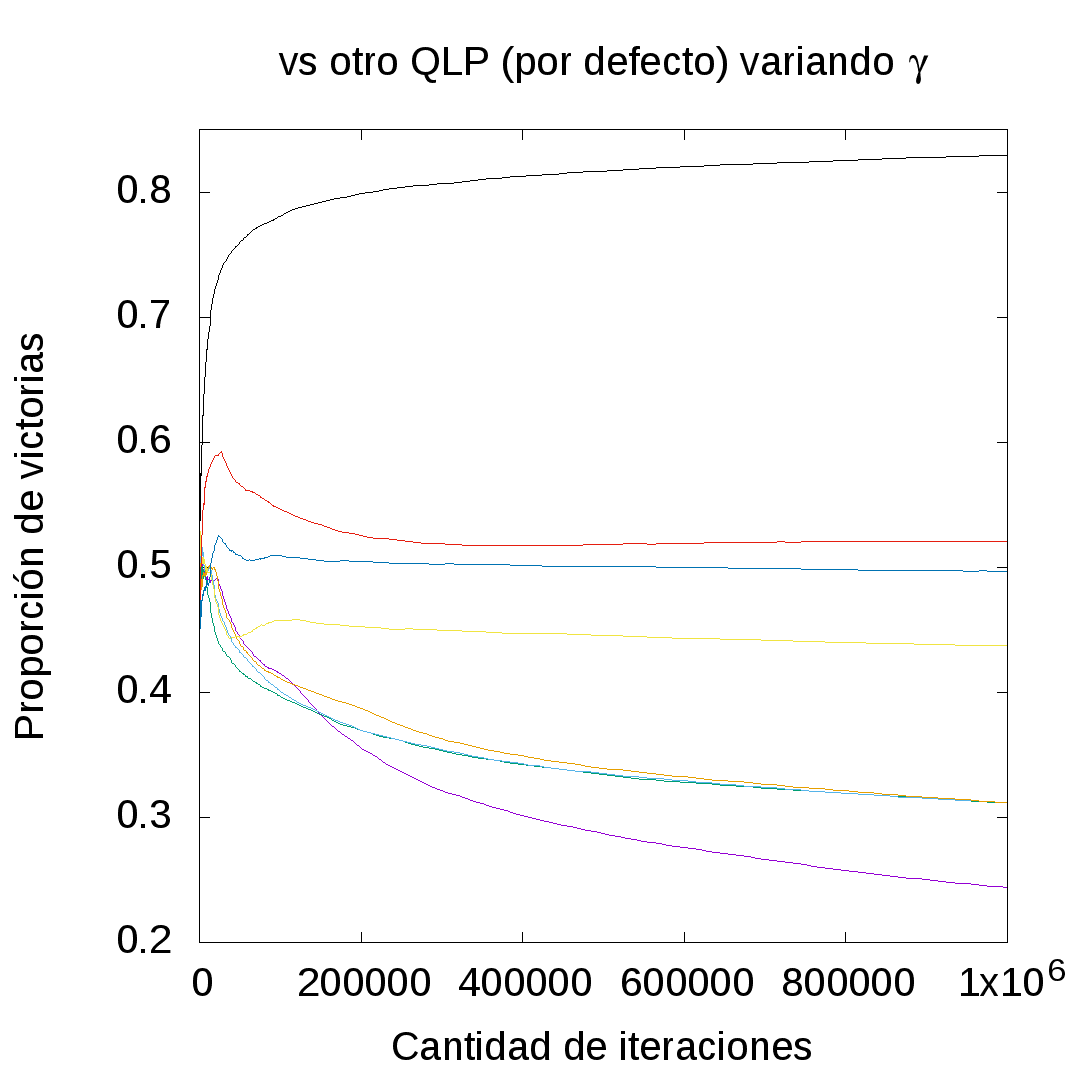
\includegraphics[scale=0.2]{GammaQ.png}
  \end{minipage}
\end{figure}

Aquí observamos que el mejor valor que puede tomar $\gamma = 1$ ya que tiene mayor cantidad de victorias y tiene un aprendizaje más rápido en ambas competencias (vs. un jugador Random y vs. otro jugador QLearner). Si bien se recomienda no usar $\gamma = 1$, en nuestro caso es posible hacerlo ya que no puede diverger el valor de Q para un estado ya que el tablero es finito.

\subsubsection{Experimentacion con Alpha}

\begin{figure}[H]
  \begin{minipage}[c]{1\textwidth}
  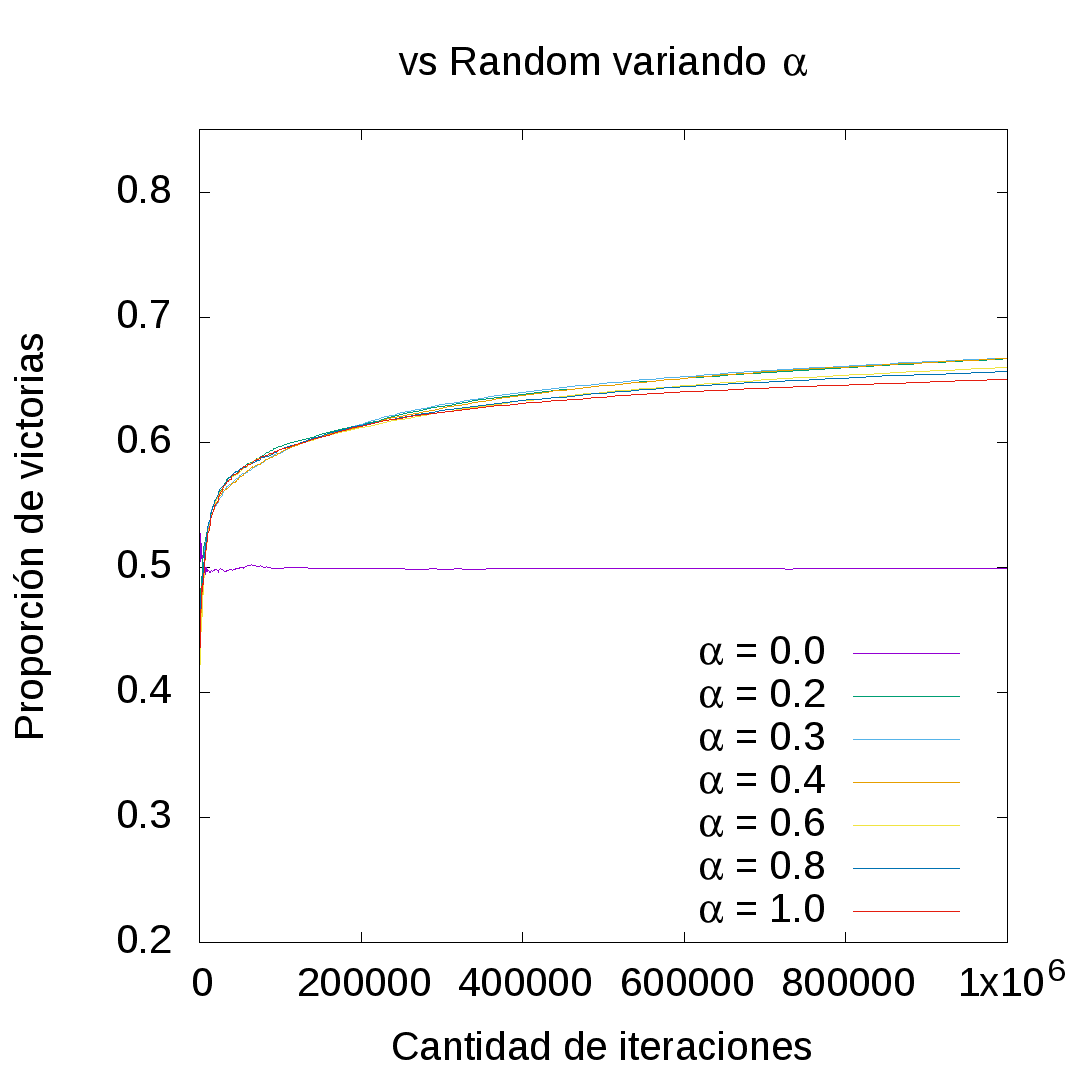
\includegraphics[scale=0.25]{AlphaR.png}
  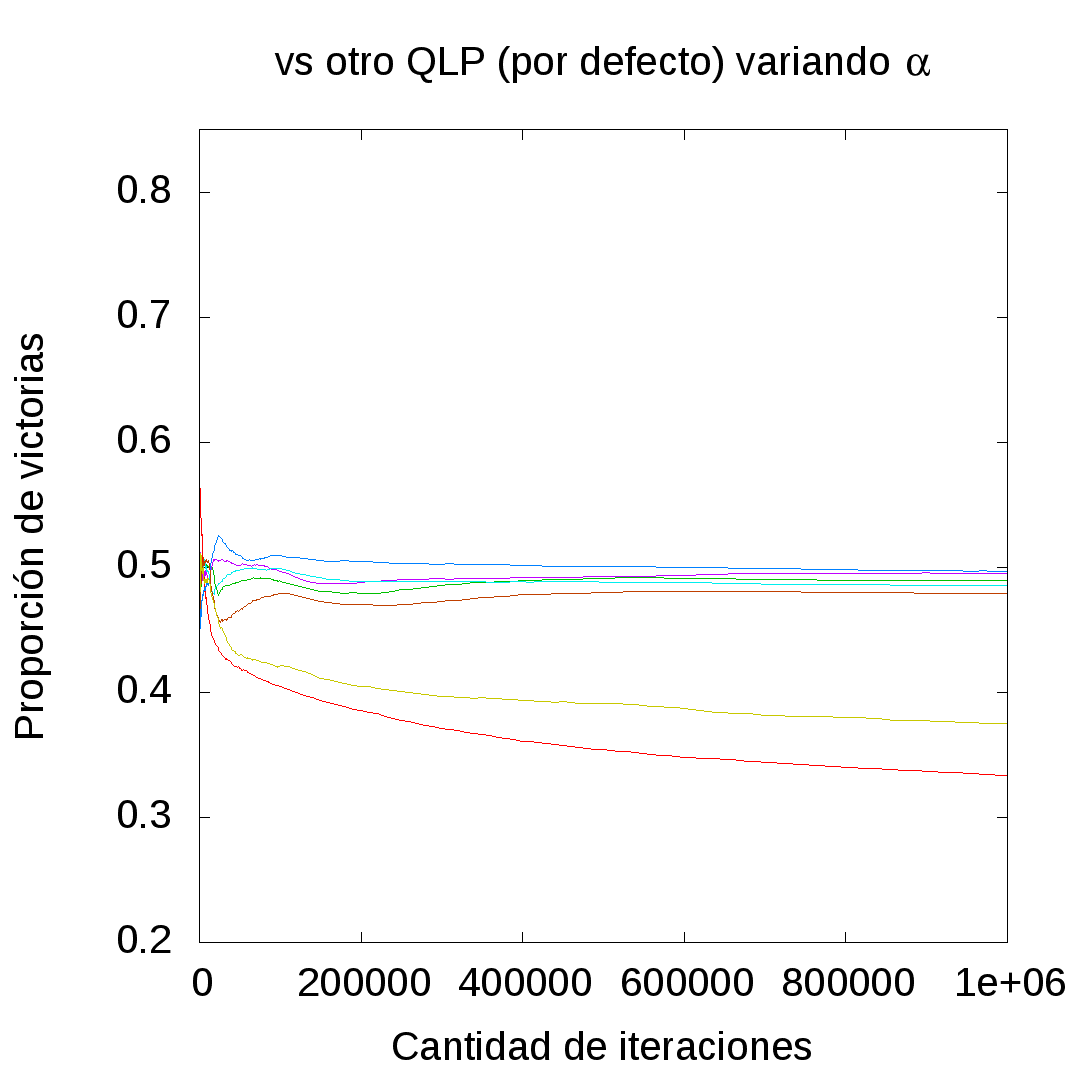
\includegraphics[scale=0.25]{AlphaQ.png}
  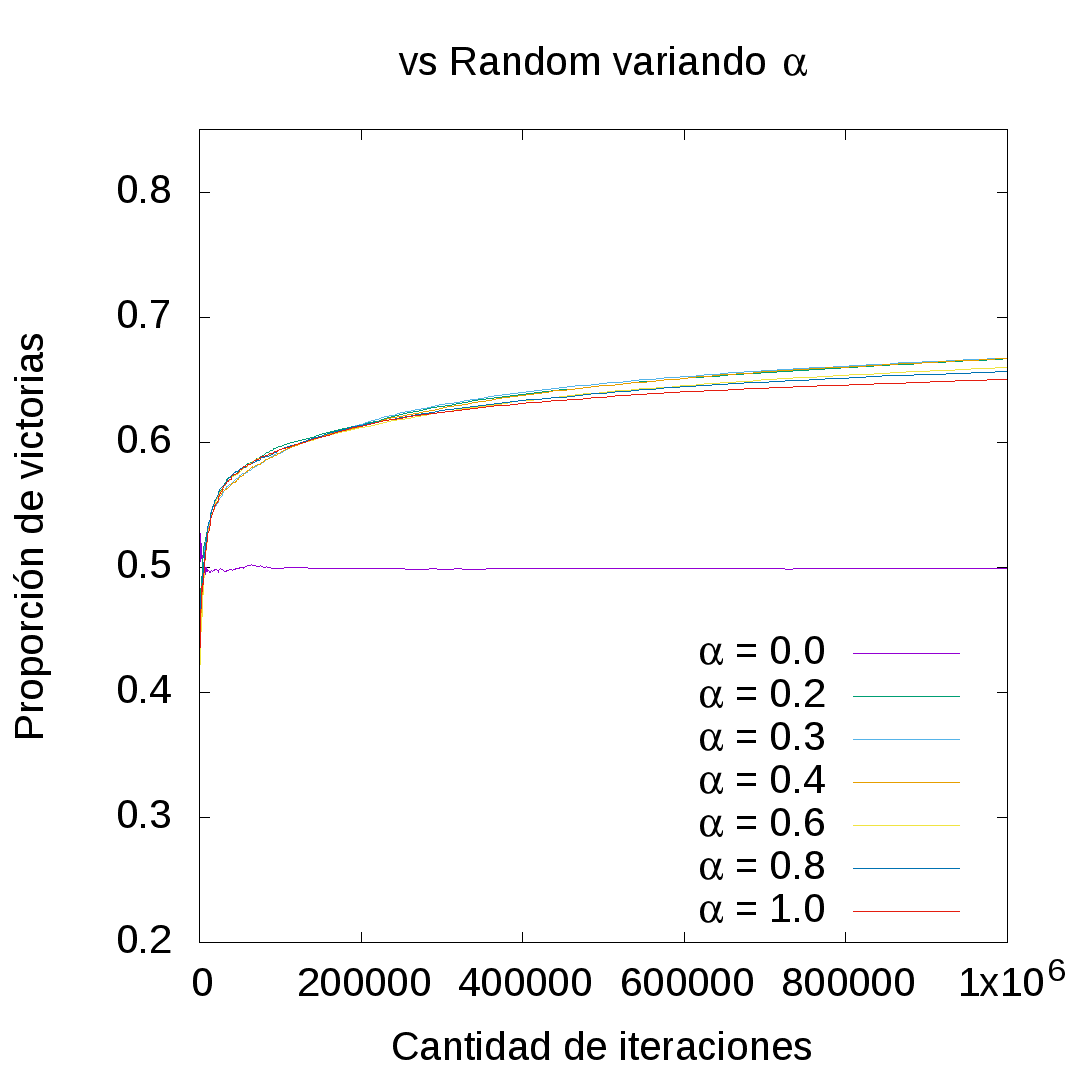
\includegraphics[trim=230mm 185mm 13mm 90mm, clip, scale=2]{AlphaR.png}
  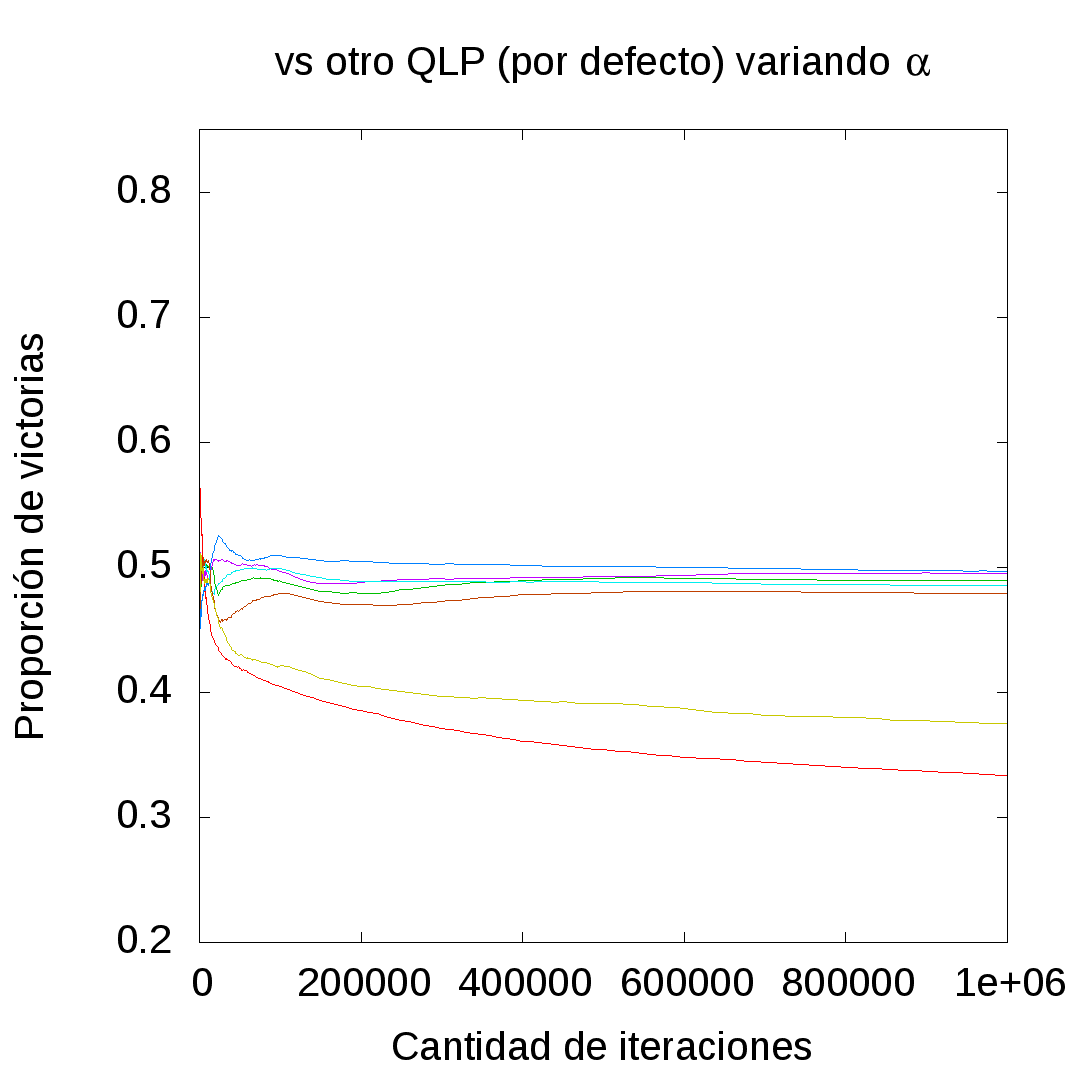
\includegraphics[trim=235mm 125mm 0mm 150mm, clip, scale=2]{AlphaQ.png}
  \end{minipage}
\end{figure}

Variando $\alpha$ hay una diferencia sútil en los distintos modelos pero el mejor valor es $\alpha=0.3$. También se puede observar que con $\alpha=0$, el modelo se comporta como un jugador Random, algo esperable ya que es el caso en que no hay exploración.

\subsubsection{Experimentacion con Epsilon}

\begin{figure}[H]
  \begin{minipage}[c]{1\textwidth}
	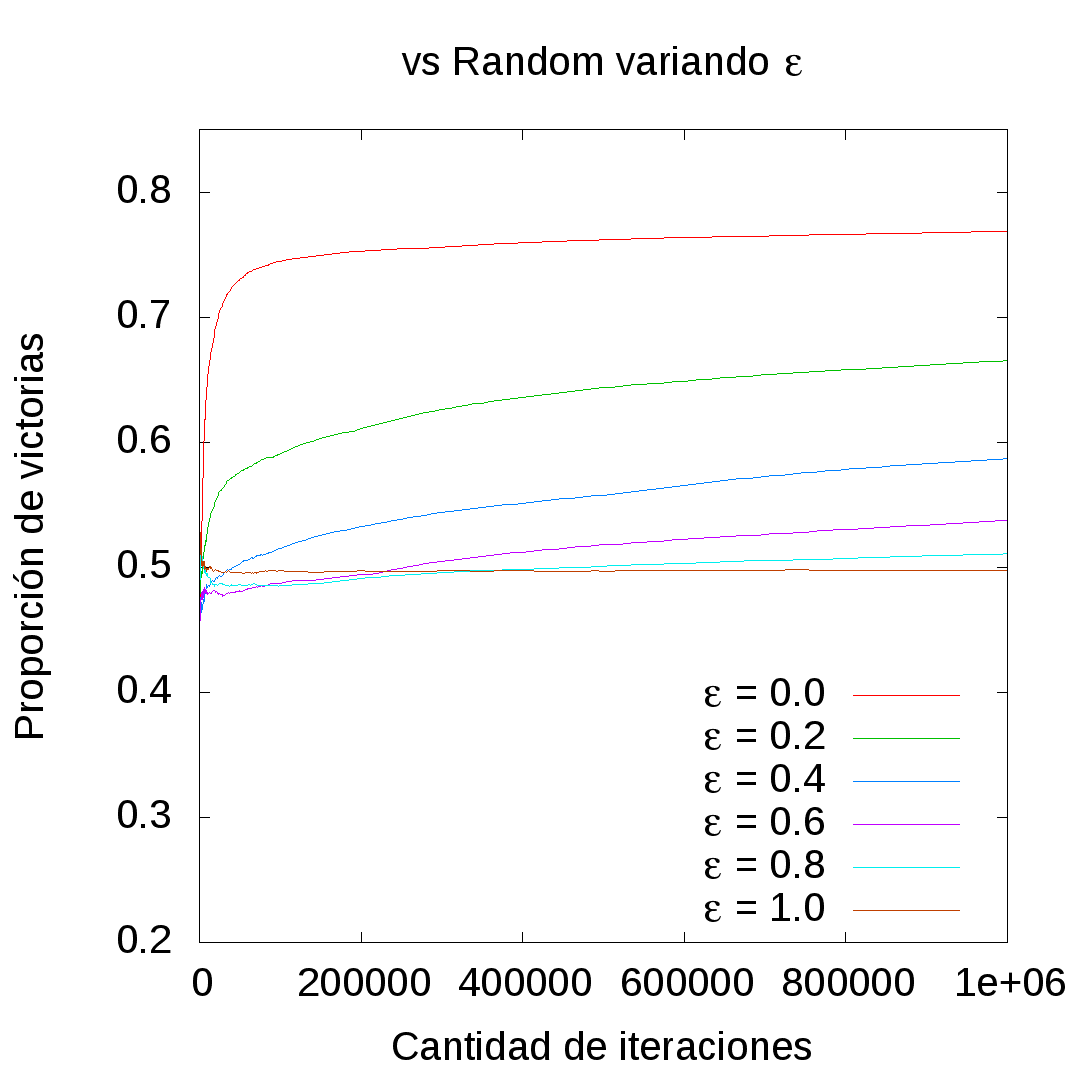
\includegraphics[scale=0.2]{EpsilonR.png}
	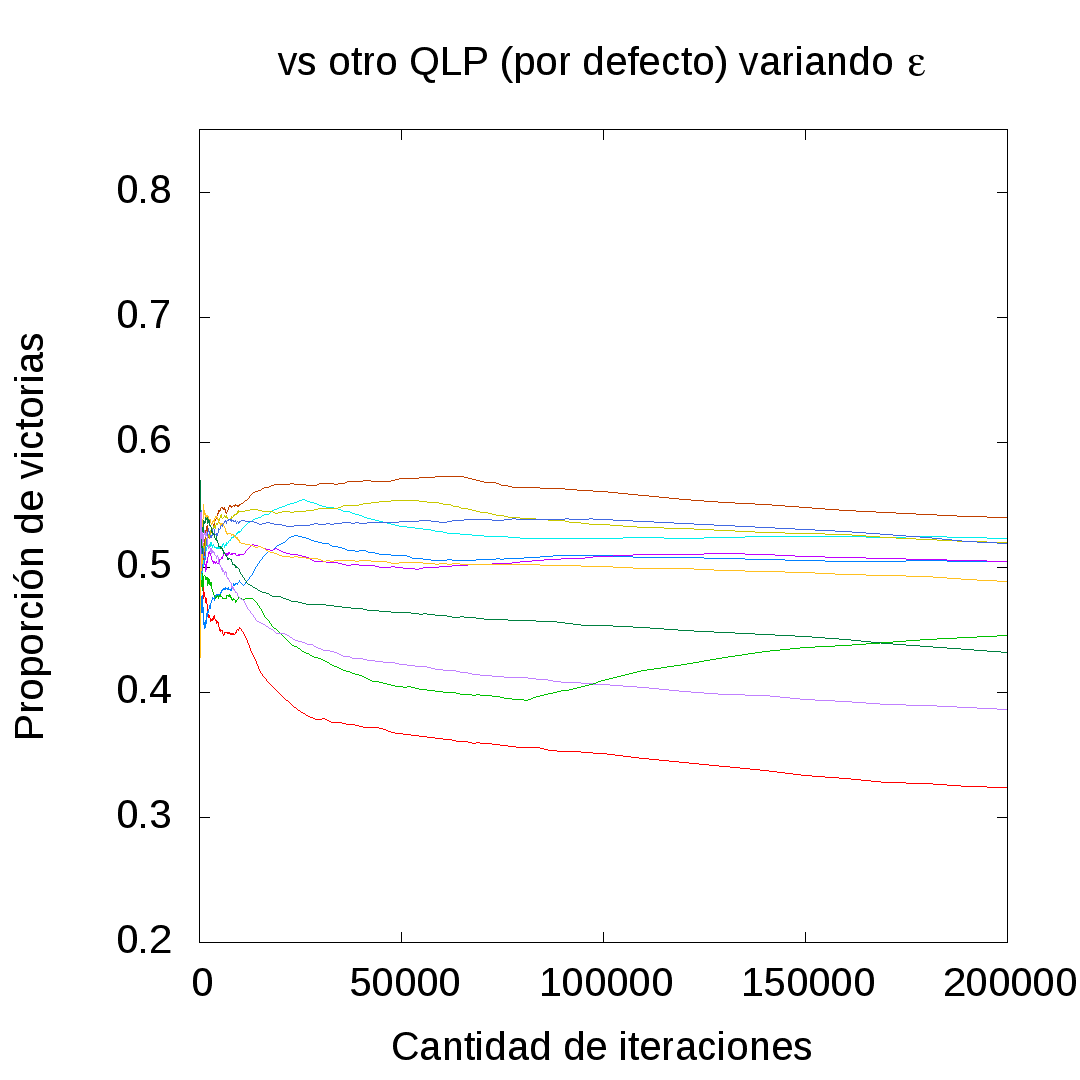
\includegraphics[scale=0.2]{EpsilonQ.png}
  \end{minipage}
\end{figure}

En este caso, no hay un claro valor óptimo. Sin embargo elegimos seguir con $\epsilon=0.2$ ya que en ambos casos termina segundo en cuanto a la cantidad de victorias después de un millón de iteraciones.

\subsection{Experimentos con parámetros ajustados}

Luego una vez que ya definidos nuestros parámetros ($\alpha=0.3$, $\gamma=1.0$, $\epsilon=0.2$) del QLP, nos pusimos a pensar en otro tipo de experimentación y nos surgieron las siguientes dudas, algunas de ellas fueron:\\
¿Cuándo se genera un mejor jugador QLearner? \\
¿Cuándo es mejor entrenarlo contra otro QLearner, ó contra un Random? \\
¿Cambia la performance de un jugador si se entrena en distinto orden con un Random y después con un QLearner?\\
¿Es mejor un jugador si se lo entrena con otro ``mejor''?\\

Entonces para atacar estas preguntas e intentar responderlas se nos ocurrio realizar los siguientes experimentos:

\begin{figure}[H]
  \begin{minipage}[c]{1\textwidth}
    \begin{center}
    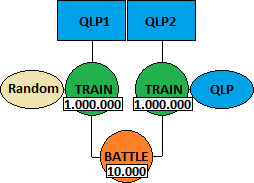
\includegraphics[scale=0.5]{E1.png}
    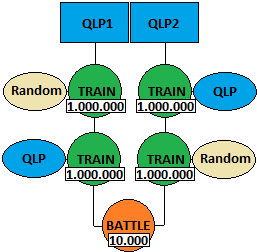
\includegraphics[scale=0.5]{E2.png}
    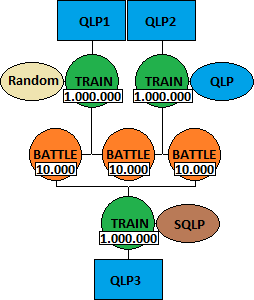
\includegraphics[scale=0.5]{E3.png}
    \end{center}
  \end{minipage}
\end{figure}

En todos los experimentos planteamos primero una fase de entrenamiento, donde entrenamos distintos QLP antes distintos jugadores, donde cada entrenamiento es de 1 millon de iteraciones y luego una fase de competencia, donde enfrentamos a los QLP entrenados entre si, cambiando los parámetros del modelo para que no aprendan mas y juegan 10 mil iteraciones.

En el primer experimento, el de la izquierda de la figura, entrenamos dos QLP uno contra otro QLP y otro contra un Random y luego compiten entre si.\\

En el segundo experimento, el del medio de la figura, extendemos el experimento anterior agrandando la fase de entrenamiento, haciendo que cada QLP entrenado vuelva a entrenar pero contra el jugador que no le habia tocado en el caso anterior. Es decir tenemos por un lado un QLP entrenado contra otro QLP y luego con un Random y por otro lado un QLP entrenado contra un Random y contra otro QLP. Luego ponemos a competir estos dos QLP entrenados.\\

Por ultimo en el tercer experimento, incluimos un nuevo tipo de jugador SmartQLearnerPlayer y hacemos una experimentacion similar al experimento uno pero agregando un QLP, que entrena contra este SQLP y luego compiten los tres QLP entre si.\\

Por un tema de simplicidad nos tomamos la libertad de abreviar los nombres de los jugadores entrenados, entonces por ejemplo al referenciar QQ, nos referimos a un QLP entrenado contra otro QLP, o por ejemplo QRQ, nos referimos a un QLP entrenado contra un Random y luego contra otro QLP y asi todas las combinaciones posibles.


\subsubsection{Experimento 1}


En este experimento, como dijimos antes, entrenamos un QLP contra un Random y lo hacemos competir contra otro QLP que fue entrenado con otro QLP:


\begin{figure}[H]
  \begin{minipage}[c]{1\textwidth}
    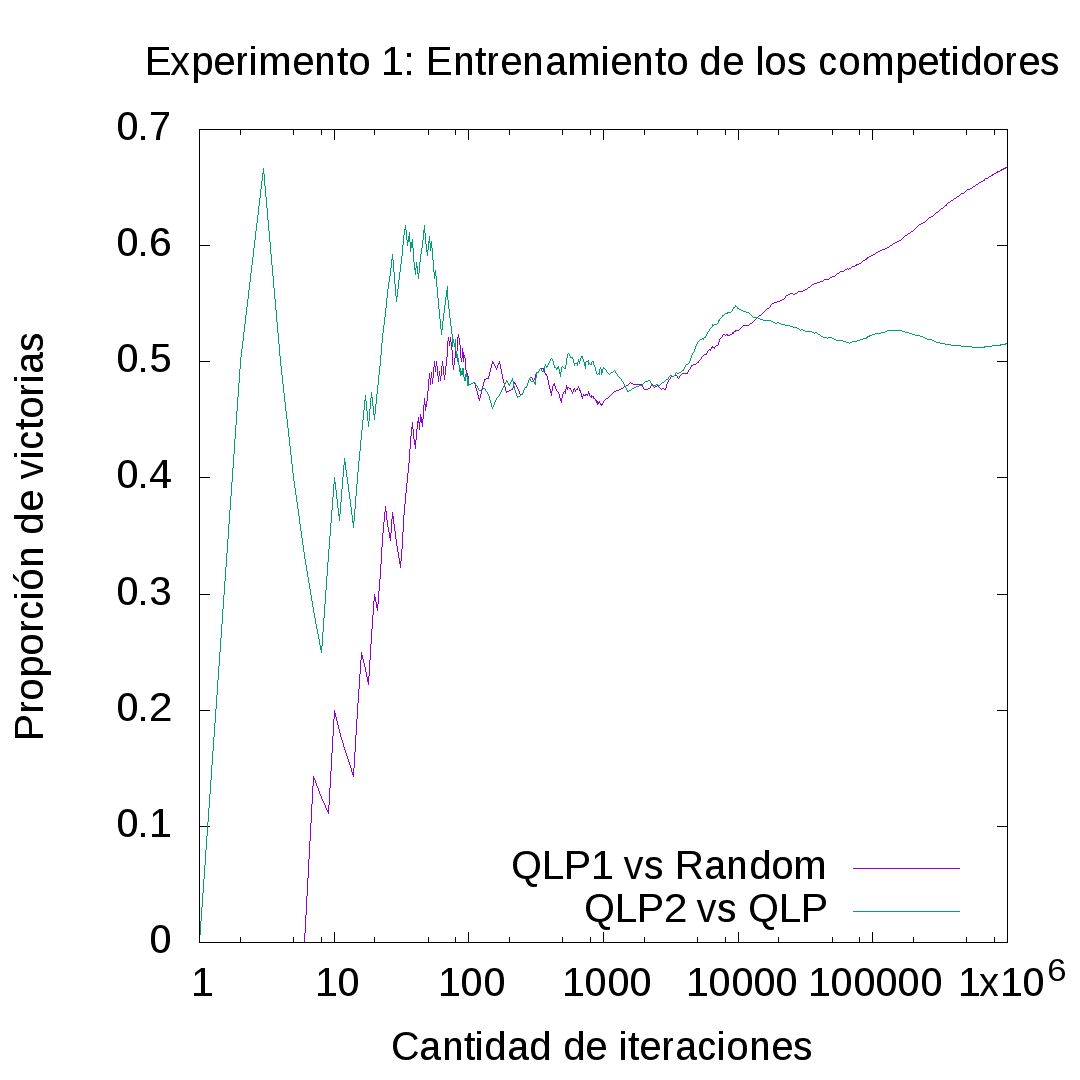
\includegraphics[scale=0.2]{E1train.png}
    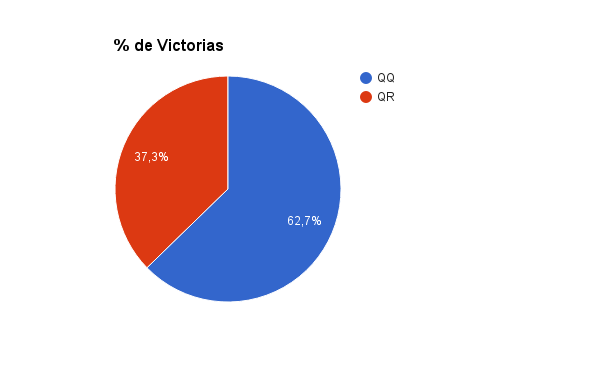
\includegraphics[scale=0.45]{QRvsQQ.png}
  \end{minipage}
\end{figure}
Aquí vemos como el QLP entrenado con otro QLearner (al que llamamos QQ) gana con una amplia diferencia. Creemos que esto se debe a que cuando se entrena con un jugador Random no puede aprender con facilidad que movimientos son buenos y cuales malos, debido a la aleatoriedad de las jugadas del Random. En cambio, el entrenado con un QLearner tiene mayor coherencia en sus movimientos y esto genera un mejor aprendizaje.

\subsubsection{Experimento 2}


En este caso queremos ver si cambia el aprendizaje según el orden de entrenamiento entre modelos. A cada modelo lo entrenamos con un Random y otro QLearner pero en distinto orden y los hacemos competir:


\begin{figure}[H]
  \begin{minipage}[c]{1\textwidth}
  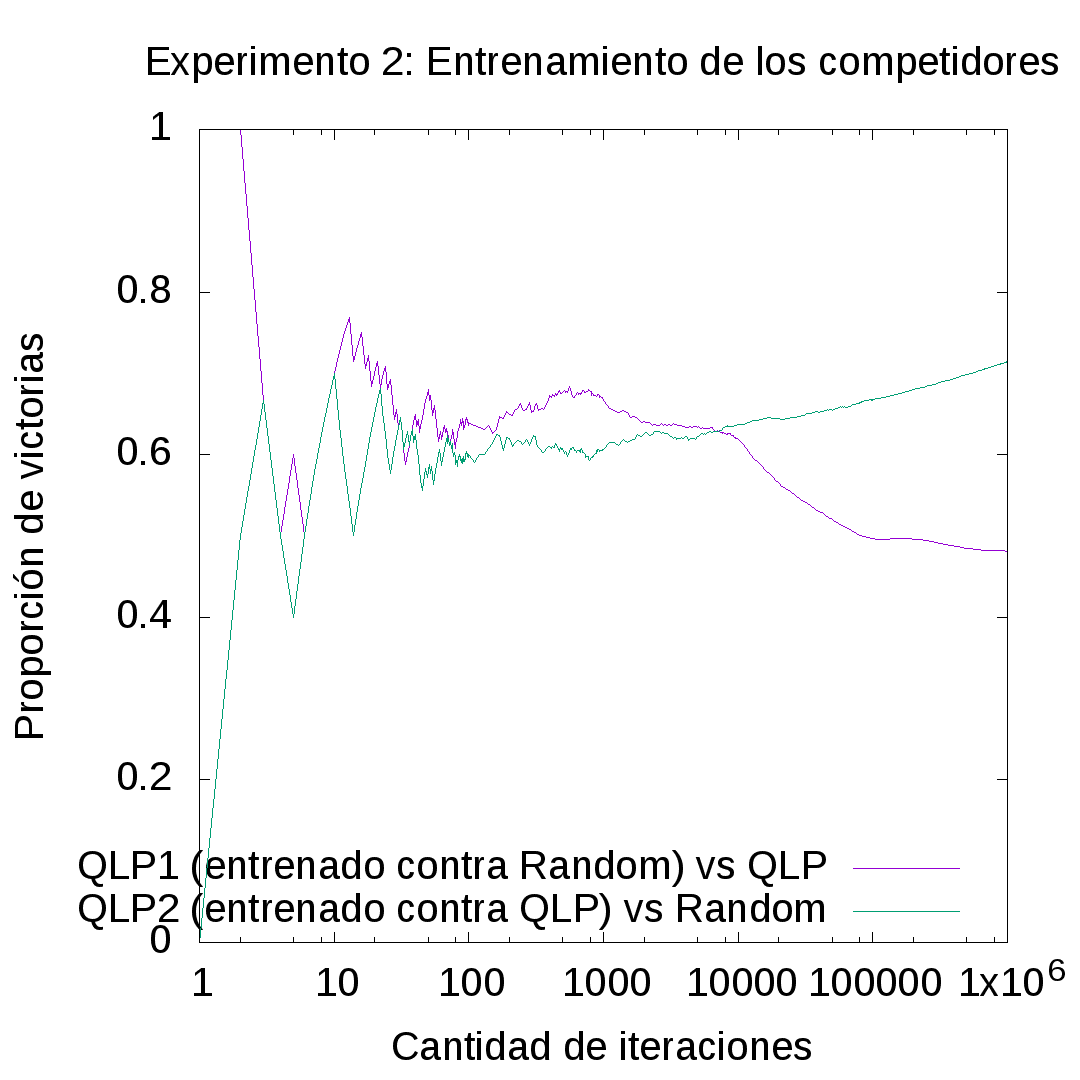
\includegraphics[scale=0.2]{E2train.png}
  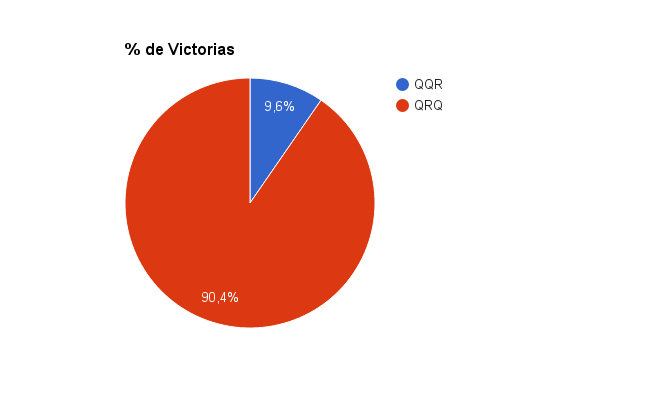
\includegraphics[scale=0.45]{QQRvsQRQ.png}
  \end{minipage}
\end{figure}

Los gráficos muestran una diferencia aún mayor entre un entrenamiento con uno Random y con un QLearner. Lo que suponemos que está generando esto es que en el entrenamiento con el Random desaprende lo visto anteriormente logrando así una peor performance.


\subsubsection{Experimento 3}

Dado que queríamos seguir mejorando el QLP, nos propusimos agregar un modelo de jugador más inteligente para que lo entrene. Realizamos entonces un jugador, que llamaremos SQLearnerPlayer o SQLP, que aprende como un QLearner pero antes de realizar una movida primero se fija si puede ganar, en ese caso inserta la ficha en la posición ganadora. En caso contrario, se fija si tiene que insertar una ficha para no perder con una jugada del rival. Si tampoco es el caso, realiza una jugada como cualquier QLearner.

En los siguientes gráficos mostramos los resultados del entrenamiento y de la competencia entre ellos:


\begin{figure}[H]
  \begin{minipage}[c]{1\textwidth}
  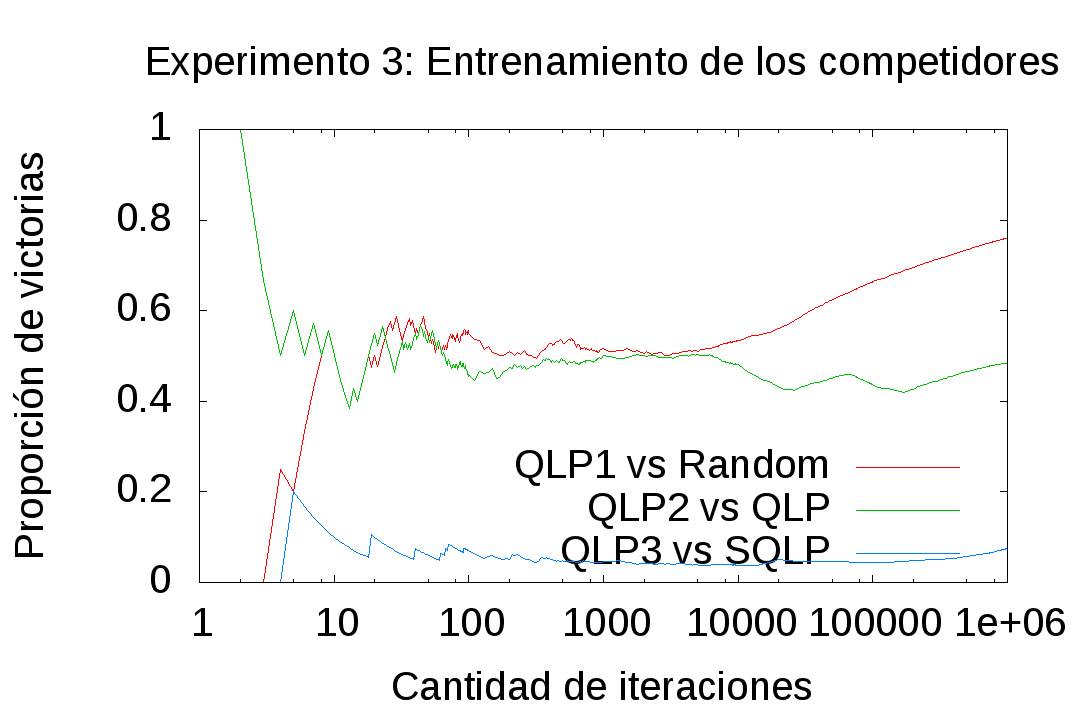
\includegraphics[scale=0.2]{E3train.png}
  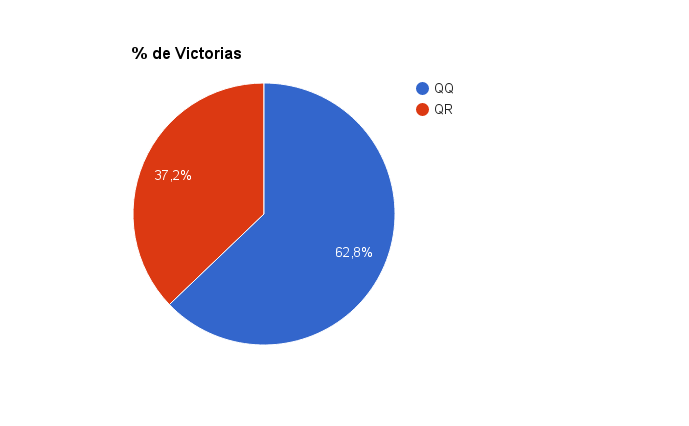
\includegraphics[scale=0.3]{QQvsQR.png}
  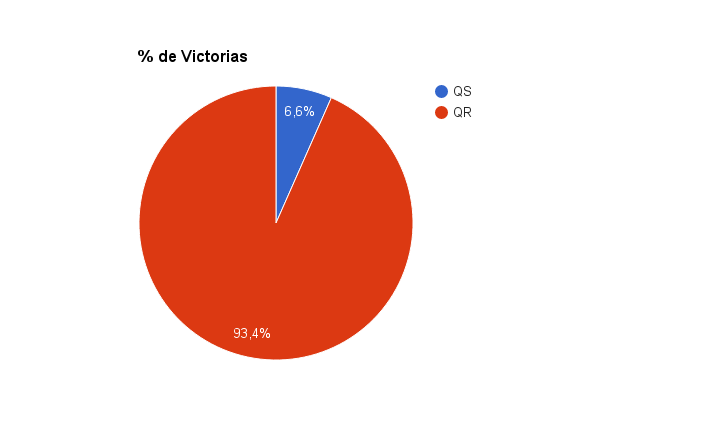
\includegraphics[scale=0.3]{QRvsQS.png}
  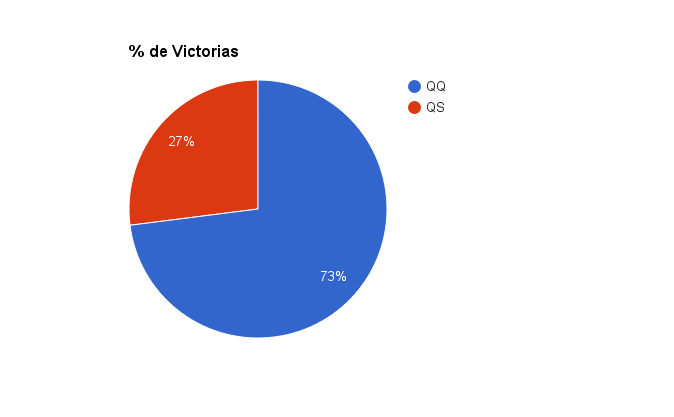
\includegraphics[scale=0.3]{QQvsQS.png}
  \end{minipage}
\end{figure}

A diferencia de nuetras expectativas entrenar un QLearner con un SQLearner dio un jugador con menos victorias. Esto creemos que se debe a que cuando se entrena con un SQLearner es muy difícil ganar y muchos movimientos se convierten en movimientos malos. En cambio, al generarse pocas victorias se tienen muy pocos movimientos con una recompensa positiva.

Otra resultado que no esperabamos, es que el jugador entrenado con Random genera más victorias que el entrenado con un QLearner cuando compiten contra el SQLearner.


%Ideas que no llegamos a hacer ???
%Contar de la idea de implementar un minimax, pero que no lo pusimos en practica porque era infinito.
%variando las recompensas?
%4x4 y ver si eso lleva a  mas empates
%comparar si cambiamos ganancia de empate a 0.
%¿juagada ganadora? Veamos si siempre empieza el jugador 1.

\section{Conclusiones}
En principio logramos ver cuáles son los parámetros óptimos para un jugador QLearner: $\alpha=0.3$,$\gamma=1$ y $\epsilon=0.2$.
Por otro lado observamos que es mejor entrenar un jugador QLearner con otro QLearner que con un jugador Random.
Si bien no pudimos obtener un jugador que sea un oponente decente para un humano, es un jugador que aprende y que le gana por una amplia diferencia a un jugador Random.


\section{Como ejecutar el tp}


En el caso en los que los valores de $\alpha$, $\gamma$ y $\epsilon$ son por defecto:
\begin{lstlisting}
python fourInLine.py key1 key2 [iteraciones]
\end{lstlisting}
donde key son los tipos de jugadores. Caso contrario: \\
\begin{lstlisting}
python fourInLine.py p key1 key2 a1 g1 e1 a2 g2 e2 rw rt rl rr save [iters]
\end{lstlisting}


\end{document}
